\subsection{Homotopy Continuation}
\label{sec:homotopy}

Homotopy continuation~\cite{HomotophyContinuationMethods} is a powerful numerical–symbolic method for solving systems of nonlinear (especially polynomial) based on a \emph{homotopy} function. The name and the intuition come from topology theory.
In topology, two continuous functions from one topological space to another are called homotopic if one can be continuously deformed into the other without breaking the continuity. In the context of polynomial systems, we can think of a polynomial system as a topological space, and a homotopy as a continuous deformation from one polynomial system to another.
The process of going from a start system to a target system is called a \emph{homotopy}, the process of tracking how solutions evolve over this homotopy is called \emph{path tracking}, and the values assumed by the system during the deformation are called \emph{solution paths}. Homotopy continuation allows us to find solutions to complex polynomial systems, starting from a simpler system with known solutions and continuously deforming it into the target system.

Formally, given a polynomial system \(F(\mathbf{x})=0\) to solve, and a polynomial system \(G(\mathbf{x})=0\) with known regular solutions \(\mathbf{x}\in\mathbb{C}^n\), a function \(H(\mathbf{x}(t),t)\) that goes from \(G\) to \(F\) is a homotopy if it satisfies

\begin{gather}
	H(\mathbf{x}(t),0)=G(\mathbf{x}(t)), \\
	H(\mathbf{x}(t),1)=F(\mathbf{x}(t)), \\
	H(\mathbf{x}(t),t) \text{ has the same number of isolated solutions } \text{ for all } t\in(0,1].
\end{gather}

A suitable choice for a homotopy function $H$ is the linear homotopy:
\begin{equation}
	H(\mathbf{x}(t),t) = (1-t)\,G(\mathbf{x}(t)) + t\,F(\mathbf{x}(t)),
	\label{eq:linear_homotopy}
\end{equation}
where \(t\in[0,1]\) is a parameter that controls the transition from \(G\) to \(F\).

We are now interested to find a solution along the path \(\mathbf{x}(t)\), such that \(H(\mathbf{x}(t),t)=0\) for \(t\in[0,1]\), shown as a solid black line in Figure~\ref{fig:homotopy_predictor_corrector}. The solution path starts at \(t=0\) with a known solution \(\mathbf{x}(0)\) of the system \(G(\mathbf{x})=0\), and ends at \(t=1\) with the searched solution \(\mathbf{x}(1)\) of the system \(F(\mathbf{x})=0\).

The most common approach is to use a predictor-corrector method, where we first predict the solution trajectory, then we correct the prediction using Newton's method to ensure that the solution satisfies \(H(\mathbf{x},t)=0\).

For our predictor step, we can use Euler's method of the second order.
To do so, we first need to differentiate Equation~\ref{eq:linear_homotopy} to form an ODE, and find the trajectory at each step
\begin{align}
\frac{\partial H}{\partial t} &= 0, \\
\frac{\partial H}{\partial \mathbf{x}} \frac{\partial \mathbf{x}}{\partial t} + \frac{\partial H}{\partial t} \frac{\partial t}{\partial t} &= 0, \label{eq:multivariable_chain_rule} \\
\frac{\partial H}{\partial \mathbf{x}} \frac{\partial \mathbf{x}}{\partial t} + \frac{\partial H}{\partial t} &= 0, \\
\frac{\partial \mathbf{x}}{\partial t} &= -\left(\frac{\partial H}{\partial \mathbf{x}}\right)^{-1} \frac{\partial H}{\partial t}. \label{eq:homotopy_derivative}
\end{align}

To compute Equation~\ref{eq:multivariable_chain_rule} we used the \emph{multivariable chain rule}, which states that the derivative of a function of multiple variables, which in turn are functions of the same underlying variable, can be expressed in terms of the sum of the standard chain rule applied to each of them. From now on the term \(\dot{\mathbf{x}} = \frac{\partial \mathbf{x}}{\partial t}\) is the derivative of the solution path \(\mathbf{x}(t)\) with respect to \(t\), and it represents the direction of the solution path at each step.

The Equation~\ref{eq:homotopy_derivative} has general validity. A specific ODE solver needs to used depending on the problem at hand. Once \(\dot{\mathbf{x}}\) is computed, we can predict the next value of \(\mathbf{x}\) as
\[
\hat{\mathbf{x}}_{k+1} = \mathbf{x}_k + \Delta t_k \dot{\mathbf{x}}_k.
\label{eq:predictor_step}
\]

As depicted in~ Figure~\ref{fig:homotopy_predictor_corrector} as a purple dotted line, our predicted solution \(\hat{\mathbf{x}}_{k+1}\) is not guaranteed to satisfy \(H(\hat{\mathbf{x}}_{k+1}, t_{k+1})=0\) due to the finite step size, so we need to correct it. Moreover perfectly satisfying \(H(\mathbf{x},t)=0\) exactly at each intermediate step is not guaranteed.
For this reason we apply Newton's method to find \(\mathbf{x}_{k+1}\) such that \(H(\mathbf{x}_{k+1}, t_{k+1})=0\) starting from the predicted value \(\hat{\mathbf{x}}_{k+1}\). We start from $\mathbf{x}_{k+1} = \hat{\mathbf{x}}_{k+1}$ and iteratively update it using:
\[
\mathbf{x}_{k+1} = \hat{\mathbf{x}}_{k+1} - \frac{\frac{\partial H}{\partial \mathbf{x}}(\hat{\mathbf{x}}_{k+1}, t_{k+1})}{H(\hat{\mathbf{x}}_{k+1}, t_{k+1})}.
\label{eq:newton_update}
\]
\emph{Newton–Raphson method} states that at each iteration this is a better approximation of the initial solution. We iterate until the residual \(H(\mathbf{x}_{k+1}, t_{k+1})\) is small enough, i.e., \(|H(\mathbf{x}_{k+1}, t_{k+1})| < \varepsilon \). This is called \(\varepsilon\)-tube in Figure~\ref{fig:homotopy_predictor_corrector}.
The blue dashed line in Figure~\ref{fig:homotopy_predictor_corrector} illustrates moving $\hat{\mathbf{x}}_{k+1}$ to $\mathbf{x}_{k+1}$ via this method.
If after a certain number of iterations the residual is still too large, the path is halted and another is tested.

\vspace{\baselineskip}

Algorithm~\ref{alg:homotopy_path_tracking} summarizes a Homotopy continuation iteration.
Starting from a known solution \(\mathbf{x}(0)\) (line 2), we numerically follow the curve \(\mathbf{x}(t)\) satisfying \(H(\mathbf{x}(t), t)=0\) from $t=0$ to $t=1$ (line 3).
Using \ref{eq:homotopy_derivative}, we compute the direction of the solution path at each step. That can be solved using any ODE method, such as Euler's method or Runge-Kutta methods (line 4).
We compute the new value of \(\mathbf{x}\) at \(t+\Delta t\) by using a prediction step (line 5) like \ref{eq:predictor_step}.
Then we correct the prediction using Newton’s method \ref{eq:newton_update} making it consistent with \(H(\mathbf{x}, t+\Delta t)=0\) (lines 7-10).
If the residual \(H(\mathbf{x}_{k+1}, t_{k+1})\) is still too large after a certain number of iterations, we halt the path and try another (lines 11-13).
We then iterate the process until we reach $t=1$.

\begin{figure}[H]
	\centering
	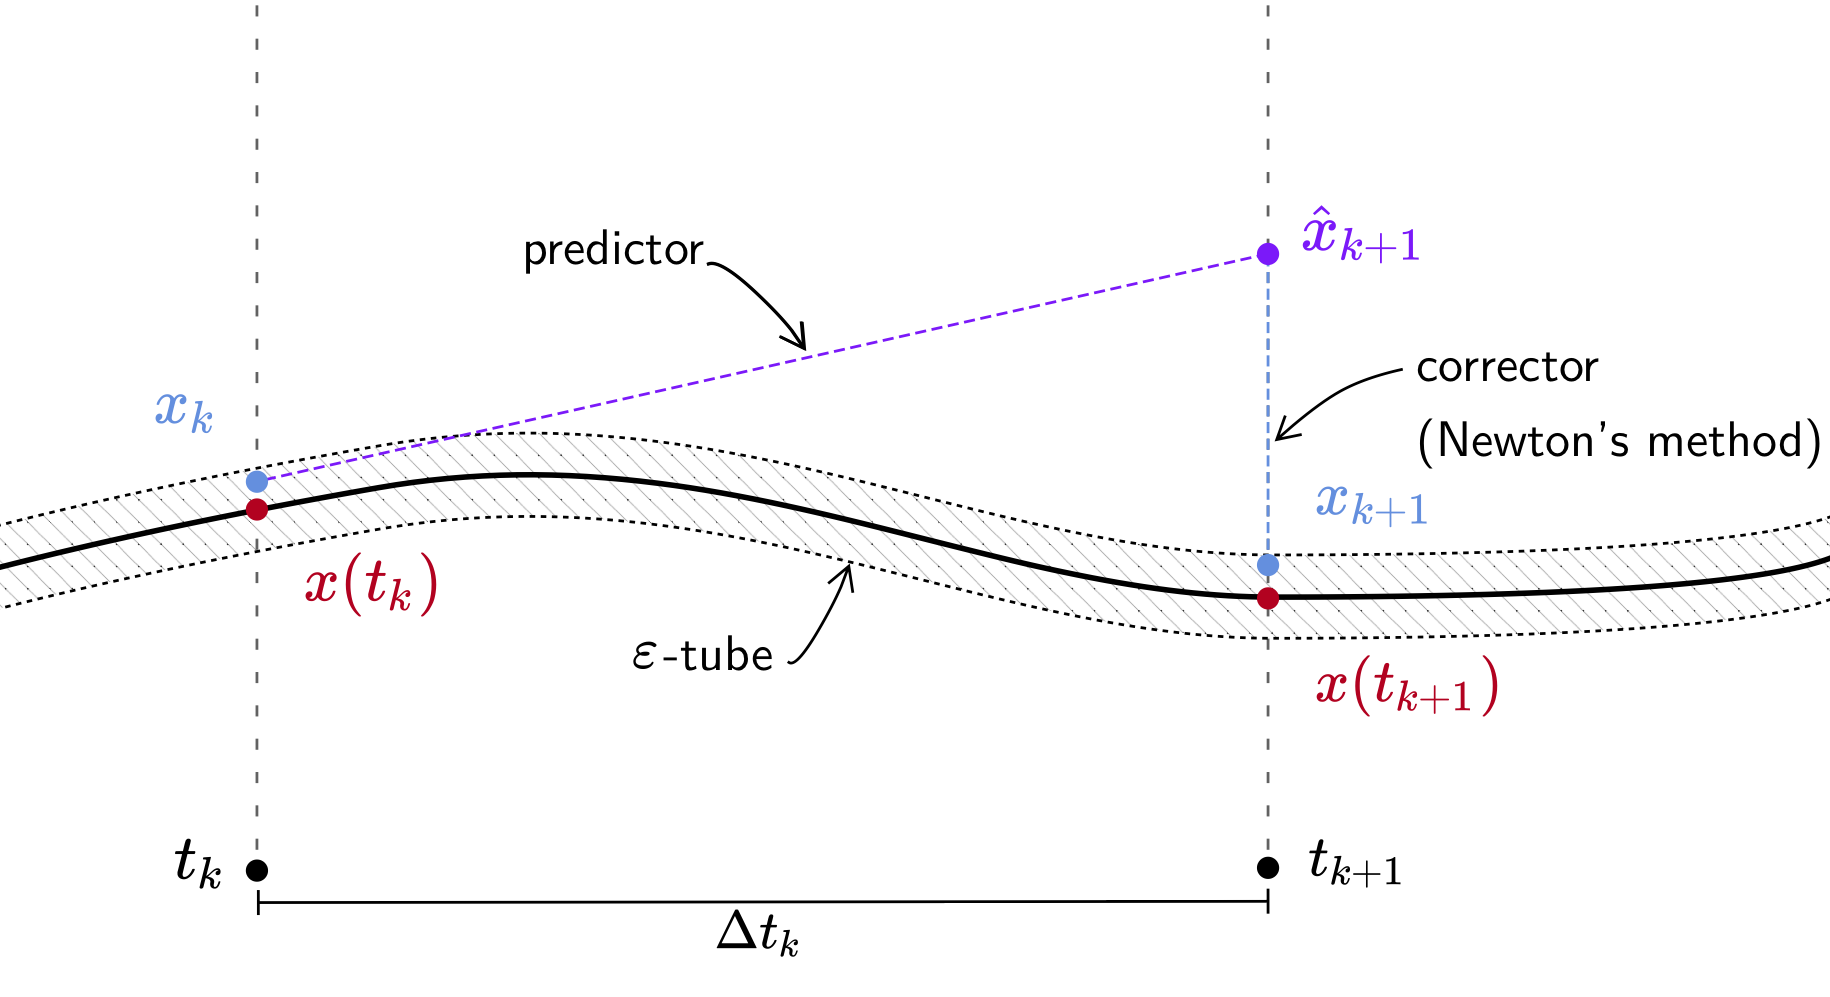
\includegraphics[width=0.85\linewidth]{images/homotopy_predictor_corrector}
	\caption{A sketch of the predictor-corrector method. In solid black the real unknown path of the solution space \(\mathbf{x}(t)\) obtained during the homotopy deformation. From the current solution \(\mathbf{x}(t_k)\), we compute the derivative \(\dot{\mathbf{x}}_k\) using \ref{eq:homotopy_derivative} at time \(t_k\) using any ODE method. We compute a prediction \(\hat{x} = x_k + \Delta t\,\dot x_k\) (purple line). More likely than not the prediction will not satisfy \(H(\hat{x}, t_k + \Delta t) = 0\). Newton's method is then used to correct the prediction, moving it to \(x_{k+1}\) (blue line) such that \(|H(x_{k+1}, t_k + \Delta t)| < \varepsilon\) is inside the \(\varepsilon\)-tube. The process is repeated until we reach \(t=1\).}
	\label{fig:homotopy_predictor_corrector}
\end{figure}

% Algorithm: Homotopy Path Tracking (Predictor-Corrector Loop)
\begin{algorithm}[H]
\caption{Homotopy Path Tracking via Predictor-Corrector}
\label{alg:homotopy_path_tracking}
\begin{algorithmic}[1]
\REQUIRE Initial solution $x_0$, step size $\Delta t$
\STATE $k \gets 0$
\STATE $x_k \gets x_0$
\WHILE{$t_k < 1$}
    \STATE $\dot x_k \gets -\left(\frac{\partial H}{\partial x}(x_k, t_k)\right)^{-1} \frac{\partial H}{\partial t}(x_k, t_k)$
    \STATE $\tilde x \gets x_k + \Delta t\,\dot x_k$ \; (Predictor: Euler or higher order)
	\STATE $x_{k+1} \gets \tilde x$ \; (Initial guess for Newton's method)
	\FOR{$\var{i} < \var{max\_iterations}$}
    	\STATE $x_{k+1} \gets x_{k+1} - \frac{H(x_{k+1}, t_{k+1})}{\frac{\partial H}{\partial x}(x_{k+1}, t_{k+1})}$ \; (Newton's update)
		\STATE $\var{i} \gets \var{i}+1$
	\ENDFOR
	\IF{$|H(x_{k+1}, t_{k+1})| > \varepsilon$}
		\RETURN null (Path halted, try another)
	\ENDIF
    \STATE $k \gets k+1$
\ENDWHILE
\RETURN $x_{k+1}$ (approximate solution to $F(x)=0$)
\end{algorithmic}
\end{algorithm}

\subsection {Parametric Homotopy}
\label{sec:parametric_homotopy}
Homotopy continuation does not require polynomial systems $F(\mathbf{x})$, $G(\mathbf{x})$ to be from the same family. However in many practical applications, including our camera calibration and pose estimation scenario, a problem can be seen as an instance of a family. Instances of the same family share the same equations degree for each, the same number of variables, and the same number of equations, but differ based on the equations coefficients. If this is the case, and we can easily find a solution for an initial set of coefficients $\mathbf{p}_0$, we can instead define a homotopy:
\[
H(\mathbf{x}, \mathbf{p}, t) = \mathcal{S}(\mathbf{x}; (1-t)\mathbf{p}_0 + t\mathbf{p}_1) = 0.
\]

Where using the previous \emph{Homotopy} notation the starting system $G(\mathbf{x}) = \mathcal{S}(\mathbf{x}; \mathbf{p}_0)$ and the target system $F(\mathbf{x}) = \mathcal{S}(\mathbf{x}; \mathbf{p}_1)$ are two instances of the same polynomial system $\mathcal{S}(\mathbf{x}; \mathbf{p})$, but with different coefficients $\mathbf{p}_0$ and $\mathbf{p}_1$. The homotopy deformation is done in the parameter space, allowing us to explore how solutions change as we vary the coefficients. Solutions can be tracked with the same methods as before.

This is called a \emph{\textbf{parametric homotopy}} and it allows us to track solutions as the parameters \(\mathbf{p}\) vary from \(\mathbf{p}_0\) to \(\mathbf{p}_1\). The parameter \(\mathbf{p}\) can be thought of as a vector of coefficients that define the specific instance of the polynomial system. \emph{Parametric homotopy} has the advantage to never leave the family of problems we are interested in, thus being geometrically consistent during the whole deformation.

We will first explain the method under a simplified problem. The reason for this is that higher dimensionality problems are harder to visualize once projected into a family.
We go deeper into defining the \emph{parametric homotopy} for our case in chapter~\ref{sec:silhouette-based-homotopy} after explaining the specific system of equations we are dealing with in chapter~\ref{sec:constraints}.

First let's discuss the relation between an equation family and its instances.
The family of $x$-centered parabolas can be represented by the equation
\[
y = p_1 x^2 + p_3,
\]
where \(p_1\) and \(p_3\) are parameters that define the amplitude and position of the parabola. By varying these parameters, we can obtain different instances of the parabola family. For the $p_0=1$, $p_3=0$ case, we have the standard parabola \(y = x^2\) with known intersection with the x-axis at the origin (Figure~\ref{fig:parametric_homotopy_original}). 
By varying the parameter \(p_3\), we obtain a surface made of parabolas translated vertically, as shown in Figure~\ref{fig:parametric_homotopy_family}. The red $x$ axis represents the function at different unknown values, the green $y$ axis represents the function deforming at varying $p_3$, and the blue line shows the solution space.

Suppose that now we want to compute the intersections of two parabolae curves, represented in Figure~\ref{fig:parametric_homotopy_instance1}.
The problem family can be defined as a system of polynomial equations
\[
\mathcal{S}(x; \mathbf{p}) = \begin{pmatrix}
p_1 x^2 + p_2 x + p_3 - y = 0 \\
p_4 x^2 + p_5 x + p_6 - y = 0
\end{pmatrix},
\label{eq:parametric_homotopy_system}
\]

where \(\mathbf{p} = (p_1, p_2, p_3, p_4, p_5, p_6)\) are the parameters that define the two parabola (specific instance of the system), and $x$ is the variable of interest. Changing the parameters \(\mathbf{p}\) will change the shape and position of the curves (see Figure~\ref{fig:parametric_homotopy_instance2}), thus changing the solution set of the system \(\mathcal{S}(x; \mathbf{p}) = 0\). The solution set will vary continuously as the parameters change, and we can track how the solutions evolve as we vary \(\mathbf{p}\). By just varying the parameters, we can explore a vast range of solutions from two points intersections, one tangent point, to no intersections at all.

\begin{figure}[hb]
	\centering
	\subfloat[
		A parabola instance of the family $y = p_1 x^2 + p_3$.
	]{
		% 
\includegraphics[width=0.23\linewidth]{images/parametric_homotopy/original}
		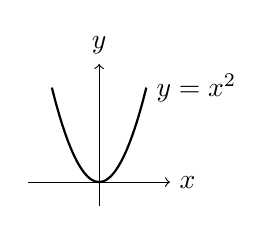
\begin{tikzpicture}[scale=0.3]
			% Draw axes
			\draw[->] (-3, 0) -- (3, 0) node[right] {$x$};
			\draw[->] (0, -1) -- (0, 5) node[above] {$y$};

			% Draw parabola y = x^2
			\draw[domain=-2:2, smooth, variable=\x, black, thick] 
				plot ({\x}, {\x*\x}) node[right] {$y = x^2$};
		\end{tikzpicture}
		\label{fig:parametric_homotopy_original}
	}
	\hspace{0.01\linewidth}
	\subfloat[
		The surface resulting from varying the parameter $p_3$. We can see that the solution set (highlighted in blue) varies continuously as the parameter (Y axis) changes.
	]{
		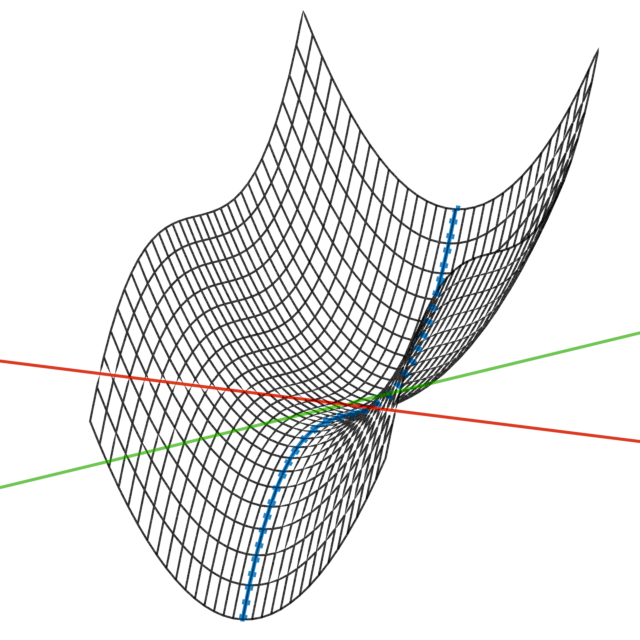
\includegraphics[width=0.23\linewidth]{images/parametric_homotopy/family_surface.png}
		\label{fig:parametric_homotopy_family}
	}
	\hspace{0.01\linewidth}
	\subfloat[
		An instance of the polynomial system $F(x; p) = 0$ with $p = (1, 0, 0, -1, 0, 0)$.
	]{
		% 
\includegraphics[width=0.23\linewidth]{images/parametric_homotopy/instance1}
		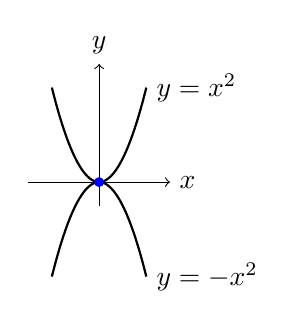
\begin{tikzpicture}[scale=0.3]
			% Draw axes
			\draw[->] (-3, 0) -- (3, 0) node[right] {$x$};
			\draw[->] (0, -1) -- (0, 5) node[above] {$y$};

			% Draw parabola y = x^2
			\draw[domain=-2:2, smooth, variable=\x, black, thick] 
				plot ({\x}, {\x*\x}) node[right] {$y = x^2$};
			% Draw parabola y = -x^2
			\draw[domain=-2:2, smooth, variable=\x, black, thick] 
				plot ({\x}, {-\x*\x}) node[right] {$y = -x^2$};

			% Draw intersection points
			\fill[blue] (0, 0) circle (6pt) node[below right] {};
		\end{tikzpicture}
		\label{fig:parametric_homotopy_instance1}
	}
	\hspace{0.01\linewidth}
	\subfloat[
		An instance of the polynomial system $F(x; p) = 0$ with $p = (1, 0, 1, -1, 0, -1)$.
	]{
		% 
\includegraphics[width=0.23\linewidth]{images/parametric_homotopy/instance2}
		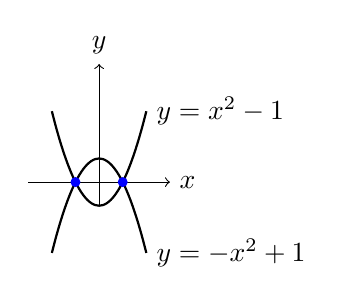
\begin{tikzpicture}[scale=0.3]
			% Draw axes
			\draw[->] (-3, 0) -- (3, 0) node[right] {$x$};
			\draw[->] (0, -1) -- (0, 5) node[above] {$y$};

			% Draw parabola y = x^2 - 1
			\draw[domain=-2:2, smooth, variable=\x, black, thick] 
				plot ({\x}, {\x*\x - 1}) node[right] {$y = x^2 - 1$};
			% Draw parabola y = -x^2 + 1
			\draw[domain=-2:2, smooth, variable=\x, black, thick] 
				plot ({\x}, {-\x*\x + 1}) node[right] {$y = -x^2 + 1$};

			% Draw intersection points
			\fill[blue] (1, 0) circle (6pt) node[below right] {};
			\fill[blue] (-1, 0) circle (6pt) node[below left] {};
		\end{tikzpicture}
		\label{fig:parametric_homotopy_instance2}
	}
	\caption{Parametric homotopy in polynomial systems. The first image shows a parabola instance of the family $y = p_1 x^2 + p_3$, the second shows the surface resulting from varying the parameter $p_3$, and the third and fourth images show two instances of the polynomial system $F(x; \mathbf{p}) = 0$ with different parameter values.}
\end{figure}

If for any parameter set $\mathbf{p}_0$ a solution $x_0$ is known, we can construct from \ref{eq:parametric_homotopy_system} a \emph{parametric homotopy} to track solutions as the parameters vary. In our parabola example~\ref{eq:parametric_homotopy_system}, we can take \(\mathbf{p}_0 = (1, 0, 0, -1, 0, 0)\) and \(x_0 = (0, 0)\), shown in Figure~\ref{fig:parametric_homotopy_instance1}, as a known solution with multiplicity 2. We can then track solutions as the parameters vary from \(\mathbf{p}_0\) to any other parameter set \(\mathbf{p}_1\) (e.g., \(\mathbf{p}_1 = (1, 0, 0, 1, 0, 1)\)), shown in Figure~\ref{fig:parametric_homotopy_instance2}, using again a predictor-corrector approach.

Formally, given a target polynomial system \(\mathcal{S}_1(\mathbf{x}) = \mathcal{S}(\mathbf{x}; \mathbf{p}_1)\), and a target system \(\mathcal{S}_0(\mathbf{x}) = \mathcal{S}(\mathbf{x}; \mathbf{p}_0)\) where \(\mathbf{x} \in \mathbb{C}^n\) are the unknowns, \(\mathbf{p} \in \mathbb{C}^m\) are parameters, $\mathbf{p}_0$ is a starting parameter set, and $\mathbf{p}_1$ is the target parameters set we can construct a homotopy
\[
H(\mathbf{x}, \mathbf{p}, t) = (1-t)\mathcal{S}_0(\mathbf{x}(t)) + t\mathcal{S}_1(\mathbf{x}(t)) = \mathcal{S}(\mathbf{x}(t); (1-t)\mathbf{p}_0 + t\mathbf{p}_1) = 0,
\]
where we know the starting solution $\mathbf{x}(0)$ for the starting parameter set $\mathbf{p}_0$.
We can then track solutions \(x(t)\) as \(t\) varies from \(0\) to \(1\) and \(\mathbf{p}\) varies over a path in parameter space from $\mathbf{p}_0$ to $\mathbf{p}_1$.

\subsection{Monodromy}
\label{sec:monodromy}

In problems involving polynomial systems, it is common for multiple solutions to exist, even when the system is fully determined. As of now we always supposed to have one solution $\mathbf{x}_0$ for a set of parameters \(p_0\).
For example our case of camera calibration and pose estimation, usually has 4 real solutions and 64 complex solutions, when the intrinsic matrix $\KK$ is completely unknown. However, in practice, we often only have access to one solution \(\mathbf{x}(0)\) for a given parameter set \(\mathbf{p}_0\).

This is where \emph{monodromy} becomes relevant. \emph{Monodromy} is a technique to discover new solutions from a known parameters-solution pair \(\mathbf{p}_0, \mathbf{x}(0)\).

In the context of polynomial system solving, \emph{monodromy} refers to a technique that exploits the algebraic structure of solution sets by tracking solutions under continuous deformations of the system family surface under parameter changes. In particular, when a parameterized polynomial system admits multiple solutions for generic parameter values, monodromy allows us to expand the solution set by performing loops in parameter space. It does so by observing the behaviour of the system when it "runs around" a singularity.

Consider a family of polynomial systems
\[
F(\mathbf{x}; \mathbf{p}) = 0,
\]
where \( \mathbf{x} \in \mathbb{C}^n \) are the unknowns and \( \mathbf{p} \in \mathbb{C}^m \) are parameters. Given at least one solution \( \mathbf{x}(0) \) corresponding to a parameter value \( \mathbf{p}_0 \) (Figure~\ref{fig:monodromy_original}), we project it into the surface defined by all possible parametrization~\ref{fig:monodromy_parameter_surface}, we construct a path in parameter space that starts and ends at \( \mathbf{p}_0 \) (Figure~\ref{fig:monodromy_midloop}). By numerically tracking the solution \( \mathbf{x}(0) \) along this loop (via homotopy continuation), we obtain a solution \( \mathbf{x}(1) \) at \( \mathbf{p}_0 \). In general, \( \mathbf{x}(1) \) may differ from \( \mathbf{x}(0) \), having traversed a different branch of the solution variety. Repeating this process along different loops allows the discovery of new solutions without prior knowledge of the entire solution set (Figure~\ref{fig:monodromy_conclusive}).

This method relies on the fact that the solution set over generic parameters forms a branched covering of parameter space, and monodromy paths induce permutations (forming the so-called \emph{monodromy group}) on the fiber of solutions above a generic parameter value. Under mild assumptions, if the monodromy group is transitive, sufficiently many loops will recover all solutions.

Monodromy methods serve as a valuable complement to classical homotopy continuation, especially when computing all solutions via total-degree or multihomogeneous start systems is computationally prohibitive.

For additional details on practical implementations, we refer to the monodromy functionality in

\texttt{HomotopyContinuation.jl}~\cite{HomotopyContinuationJL}.

\begin{figure}[hb]
	\centering
	\subfloat[Instance of a realization of the polynomial system family $F(\mathbf{x}; \mathbf{p}) = 0$.]{
		\begin{tikzpicture}
			\node[anchor=south west, inner sep=0] (image) at (0,0) {
\includegraphics[width=0.21\linewidth]{monodromy/original.png}};
			\begin{scope}[x={(image.south east)}, y={(image.north west)}]
				\node at (0.5, 0.17) {$F(\mathbf{x}; \mathbf{p}_0)$};
				\node at (0.5,0.47) {$\mathbf{x}_0$};
			\end{scope}
		\end{tikzpicture}
		\label{fig:monodromy_original}
	}
	\hspace{0.01\linewidth}
	\subfloat[Polynomial system family $F(\mathbf{x}; \mathbf{p}) = 0$ surface for different values of $\mathbf{p}$]{
		\begin{tikzpicture}
			\node[anchor=south west, inner sep=0] (image) at (0,0) {
\includegraphics[width=0.21\linewidth]{monodromy/parameter_surface.png}};
			\begin{scope}[x={(image.south east)}, y={(image.north west)}]
				\node at (0.5, 0.17) {$F(\mathbf{x}; \mathbf{p})$};
			\end{scope}
		\end{tikzpicture}
		\label{fig:monodromy_parameter_surface}
	}
	\hspace{0.01\linewidth}
	\subfloat[Mid-loop in parameter space.]{
		
\includegraphics[width=0.21\linewidth]{monodromy/midloop.png}
		\label{fig:monodromy_midloop}
	}
	\hspace{0.01\linewidth}
	\subfloat[Conclusive loop in parameter space. Two new solutions are found.]{
		
\includegraphics[width=0.21\linewidth]{monodromy/successful_monodromy.png}
		\label{fig:monodromy_conclusive}
	}
	\hspace{0.1cm}
	\caption{Monodromy in polynomial system solving. The first image shows a realization of the polynomial system family, the second shows the parameter surface with the known solution $\mathbf{x}(t)$ highlighted in green. After projecting the surface a circular loop in the $xp$ plane (highlighted in blue) is constructed (third image). A flat circular loop on this plane is neither flat or circular on the surface (highlighted in red), so the solution $\mathbf{x}(1)$ at the end of the loop might not be the same as $\mathbf{x}(0)$. The fourth image shows a conclusive loop in parameter space that finds two new solutions (highlighted in green).}
	\label{fig:monodromy}
\end{figure}
